% !TEX root = ./main.tex
\graphicspath{{figures_flatplate/}}% Set graphics path location

\subsection{Flat Plate}


Computations of the flow over a flat plate have been performed and validated against the results of the Blasius solution for laminar boundary layer. The flow conditions are Mach number 0.5, angle of attack $0.0\deg$ and Reynolds number based on the plate length of $1\cdot10^6$. The governing equations are the 2D Navier-Stokes equations with a constant ratio of specific heats of $1.4$ and Prandtl number of $0.72$. The dynamic viscosity is also a constant $1.827\cdot 10^{-5} Pa \cdot s$.

\begin{figure}
\begin{center}
\begin{minipage}[t]{0.48\columnwidth}
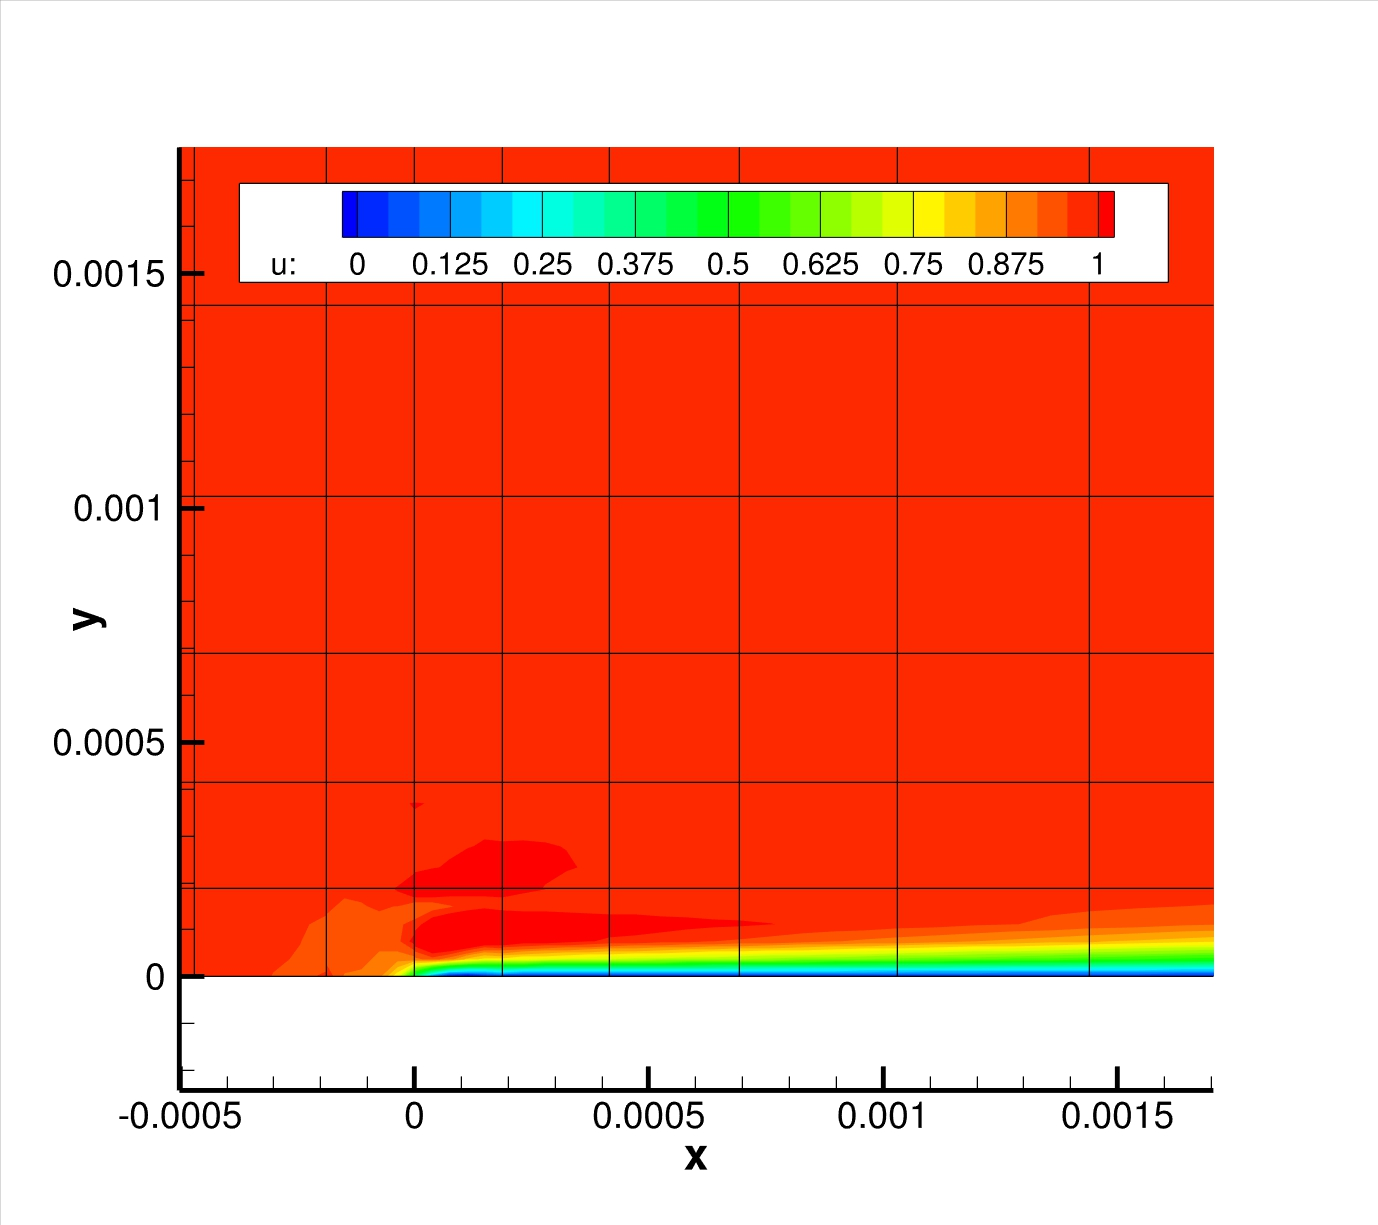
\includegraphics[width = \textwidth,clip=]{LeadingEdge.jpg}
\caption{Equivalent area distributions at different azimuth angles.}
\label{fig:Nearfield}
\end{minipage}
\hfill
\begin{minipage}[t]{0.48\columnwidth}
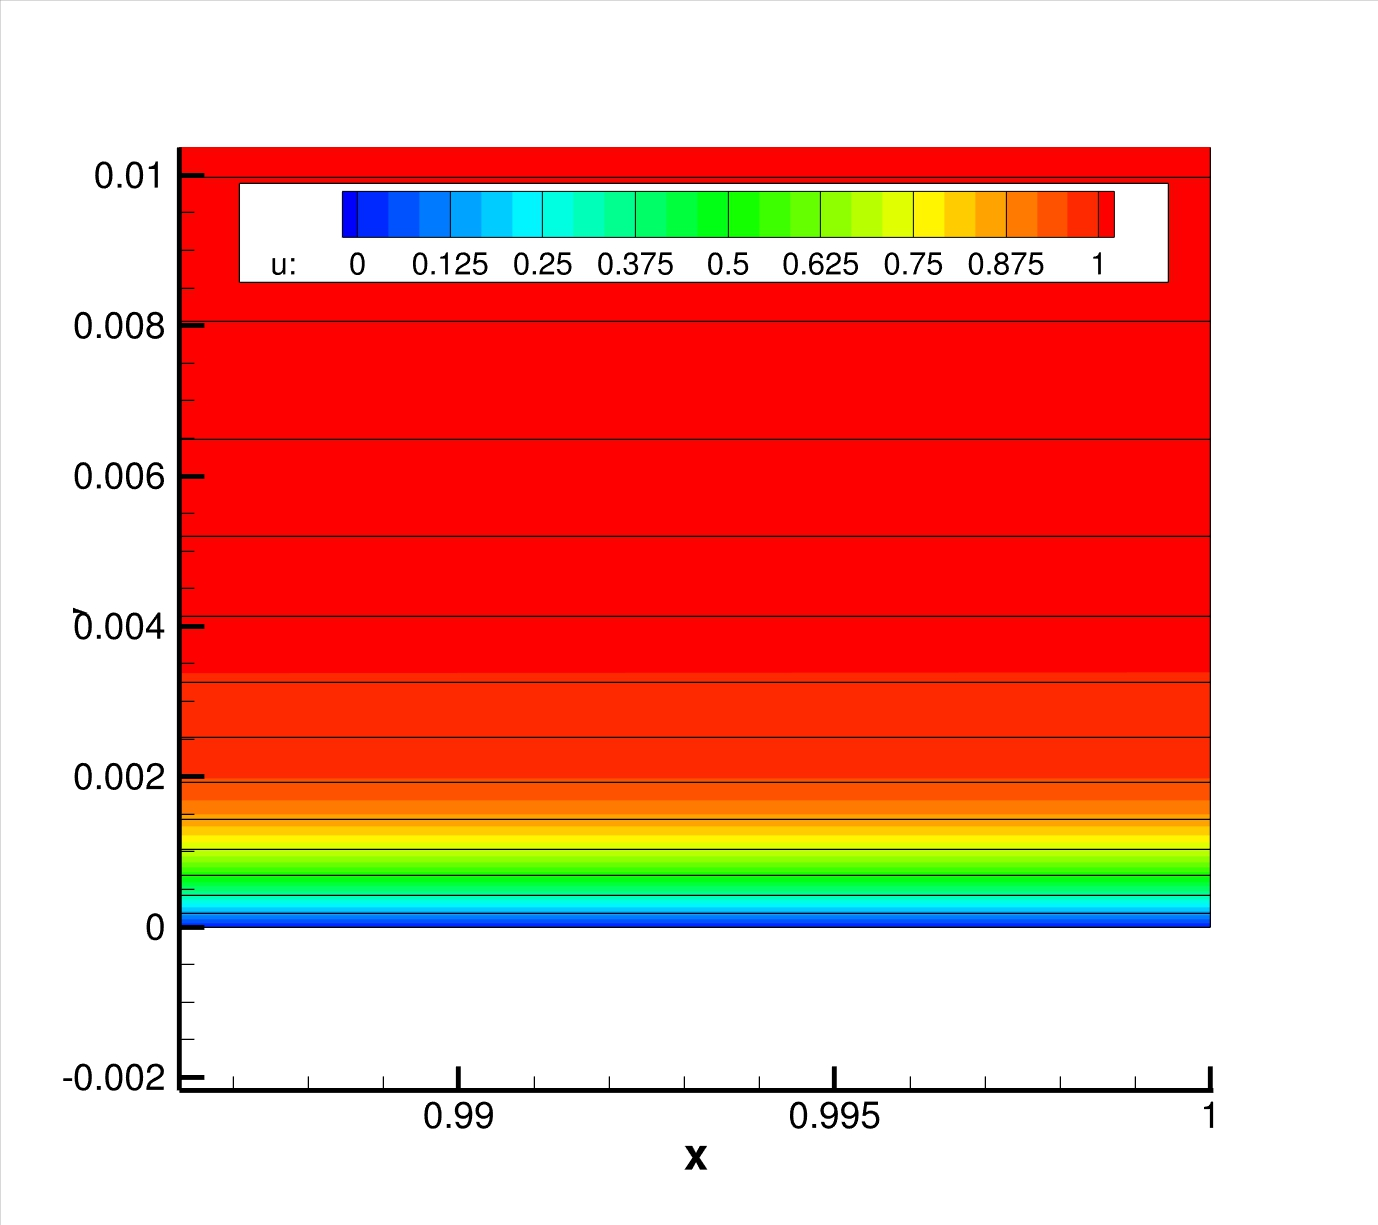
\includegraphics[width = \textwidth,clip=] {EndPlate.jpg}
\caption{Initial and final surface Contours (wing detail).}
\label{fig:DetailWing}
\end{minipage}
\end{center}
\end{figure}

The objective of this study is to determine the minimum number of elements and order of polynomial that is required to converge the simulation. In particular, 4 different grid have been used (2, 4, 6, 15 elements inside the boundary layer), and 4 order of polynomial. The results are summarized in Table ??, where it is possible to appreciate that the simulations requires a minimum number of elements in the boundary layer to obtain a satisfactory converge.

\begin{figure}
\begin{center}
\begin{minipage}[t]{0.48\columnwidth}
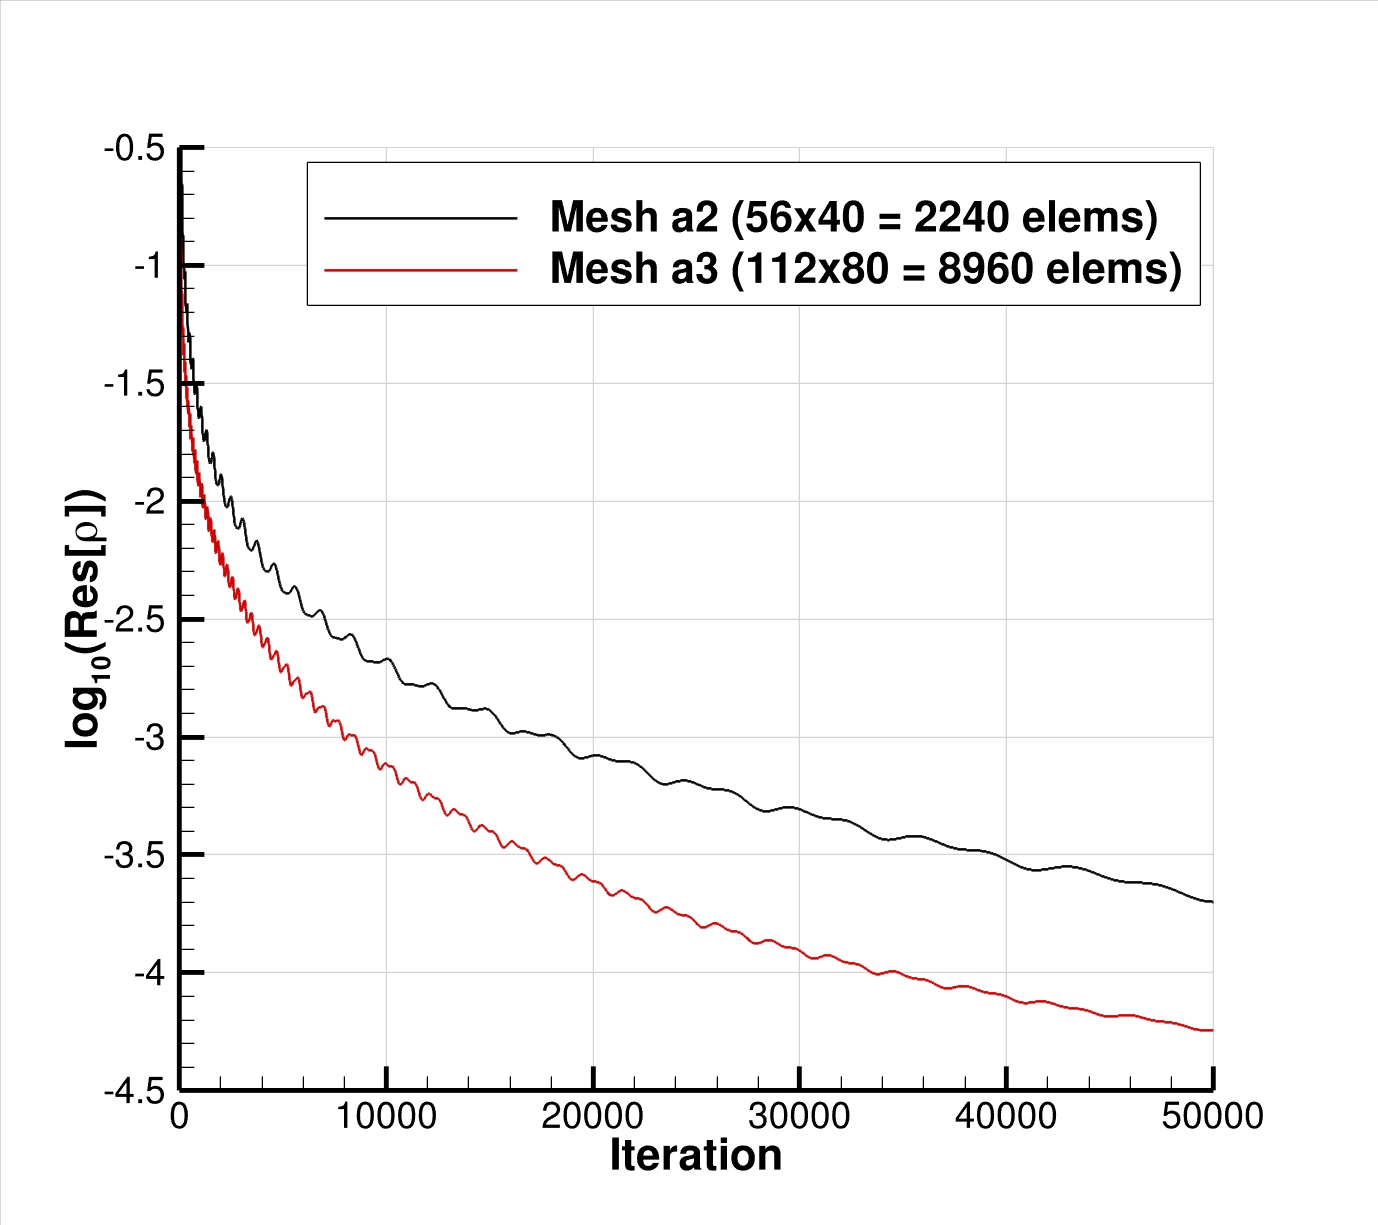
\includegraphics[width = \textwidth,clip=]{CompMesh.jpg}
\caption{Equivalent area distributions at different azimuth angles.}
\label{fig:Nearfield}
\end{minipage}
\hfill
\begin{minipage}[t]{0.48\columnwidth}
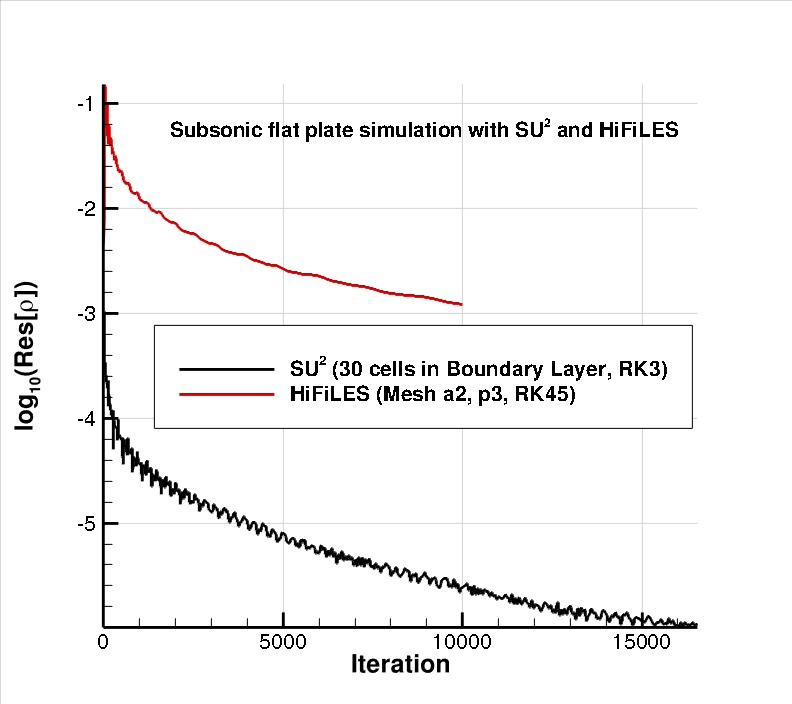
\includegraphics[width = \textwidth,clip=] {CompSu2.jpg}
\caption{Initial and final surface Contours (wing detail).}
\label{fig:DetailWing}
\end{minipage}
\end{center}
\end{figure}

On the other hand, it is important to note that the absence of a local time stepping implementation in HiFiLES increases the required number of iterations to obtain a converged solution, however, the rate of convergence is not affected by the order of the method (see Fig.\ref{}), and it is comparable to a second order numerical code running with a similar numerical scheme (see Fig.\ref{}).

\begin{center}
    \begin{tabular}{l*{5}{c}r}
    \hline
    Height first cell/ number of cells inside the boundary layer & Order 2 & Order 3 & Order 4 & Order 5 \\ \hline
    A0 (140 = 14x10) 0.00075 / 2 cells & $\times$ & $\times$ & $\times$ & \Checkmark \\ \hline
    A1 (560 = 28x20) 0.000375 / 4 cells &  $\times$ & $\times$ & \Checkmark & \Checkmark \\ \hline
    A1 (560 = 28x20) 0.000375 / 4 cells & $\times$ & \Checkmark & \Checkmark & \Checkmark \\ \hline
    A2 (2240 = 56x40) 0.000375 / 4 cells & \Checkmark & \Checkmark & \Checkmark & \Checkmark \\
    \hline
    \end{tabular}
\end{center}


